% ----------------------------------------------------------
% FIGURE: UD SHORTFALL DEPTHS
% ----------------------------------------------------------
\begin{figure}[h!]
\centering
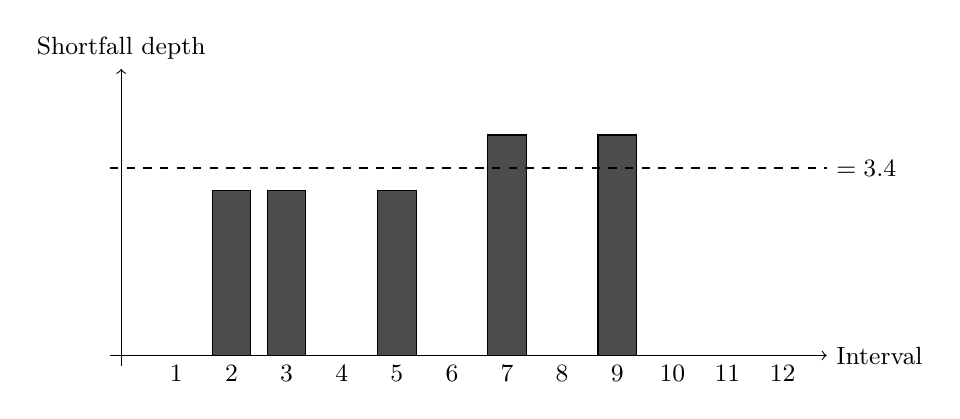
\begin{tikzpicture}[scale=0.7]

% Axes
\draw[->] (-0.2,0) -- (12.8,0) node[right] {\small Interval};
\draw[->] (0,-0.2) -- (0,5.2) node[above] {\small Shortfall depth};

% Shortfall bars (only intervals with s_t > 0)
\draw[fill=black!70] (2-0.35,0) rectangle ++(0.7,3);
\draw[fill=black!70] (3-0.35,0) rectangle ++(0.7,3);
\draw[fill=black!70] (5-0.35,0) rectangle ++(0.7,3);
\draw[fill=black!70] (7-0.35,0) rectangle ++(0.7,4);
\draw[fill=black!70] (9-0.35,0) rectangle ++(0.7,4);

% Interval labels
\foreach \t in {1,...,12} {
    \node[below] at (\t,0) {\small \t};
}

% Dashed UD line
\draw[dashed] (-0.2,3.4) -- (12.8,3.4);
\node[right] at (12.8,3.4) {\small $\UD = 3.4$};

\end{tikzpicture}
\caption{Shortfall depths across intervals for the example in
Table~\ref{tab:ud_example}. The dashed line indicates the Underbuild Depth (\UD).}
\label{fig:ud_depths}
\end{figure}